%%%%%%%%%%%%%%%%%%%%%%%%%%%%%%%%%%%%%%%%%
% Arsclassica Article
% LaTeX Template
% Version 1.1 (05/01/2015)
%
% This template has been downloaded from:
% http://www.LaTeXTemplates.com
%
% Original author: Adriano Palombo
%
%
%%%%%%%%%%%%%%%%%%%%%%%%%%%%%%%%%%%%%%%%%

%----------------------------------------------------------------------------------------
%	PACKAGES AND OTHER DOCUMENT CONFIGURATIONS
%----------------------------------------------------------------------------------------

\documentclass[
10pt, % Main document font size
a4paper, % Paper type, use 'letterpaper' for US Letter paper
oneside, % One page layout (no page indentation)
%twoside, % Two page layout (page indentation for binding and different headers)
headinclude,footinclude, % Extra spacing for the header and footer
BCOR5mm, % Binding correction
]{scrartcl}


%%%%%%%%%%%%%%%%%%%%%%%%%%%%%%%%%%%%%%%%%
% Arsclassica Article
% Structure Specification File
%
% This file has been downloaded from:
% http://www.LaTeXTemplates.com
%
% Original author:
% Lorenzo Pantieri (http://www.lorenzopantieri.net) with extensive modifications by:
% Vel (vel@latextemplates.com)
%
% License:
% CC BY-NC-SA 3.0 (http://creativecommons.org/licenses/by-nc-sa/3.0/)
%
%%%%%%%%%%%%%%%%%%%%%%%%%%%%%%%%%%%%%%%%%

%----------------------------------------------------------------------------------------
%	REQUIRED PACKAGES
%----------------------------------------------------------------------------------------

\usepackage[
nochapters, % Turn off chapters since this is an article        
%beramono, % Use the Bera Mono font for monospaced text (\texttt)
%eulermath,% Use the Euler font for mathematics
pdfspacing, % Makes use of pdftex’ letter spacing capabilities via the microtype package
dottedtoc % Dotted lines leading to the page numbers in the table of contents
]{classicthesis} % The layout is based on the Classic Thesis style

\usepackage{helvet}
\usepackage{arsclassica} % Modifies the Classic Thesis package

\usepackage[T1]{fontenc} % Use 8-bit encoding that has 256 glyphs
\usepackage[utf8]{inputenc} % Required for including letters with accents
\usepackage[english]{babel}
\usepackage{graphicx} % Required for including images
\graphicspath{{Figures/}} % Set the default folder for images

\usepackage{enumitem} % Required for manipulating the whitespace between and within lists

\usepackage{lipsum} % Used for inserting dummy 'Lorem ipsum' text into the template

\usepackage{subfig} % Required for creating figures with multiple parts (subfigures)

\usepackage{amsmath,amssymb,amsthm} % For including math equations, theorems, symbols, etc

\usepackage{varioref} % More descriptive referencing

\usepackage{adjustbox}
\usepackage{booktabs}
\usepackage{textcomp}
\usepackage{hyperref}
\usepackage{physics}


%----------------------------------------------------------------------------------------
%	THEOREM STYLES
%---------------------------------------------------------------------------------------

\theoremstyle{definition} % Define theorem styles here based on the definition style (used for definitions and examples)
\newtheorem{definition}{Definition}

\theoremstyle{plain} % Define theorem styles here based on the plain style (used for theorems, lemmas, propositions)
\newtheorem{theorem}{Theorem}

\theoremstyle{remark} % Define theorem styles here based on the remark style (used for remarks and notes)

%----------------------------------------------------------------------------------------
%	HYPERLINKS
%---------------------------------------------------------------------------------------

\hypersetup{
%draft, % Uncomment to remove all links (useful for printing in black and white)
colorlinks=true, breaklinks=true, bookmarks=true,bookmarksnumbered,
urlcolor=webbrown, linkcolor=RoyalBlue, citecolor=webgreen, % Link colors
pdftitle={}, % PDF title
pdfauthor={\textcopyright}, % PDF Author
pdfsubject={}, % PDF Subject
pdfkeywords={}, % PDF Keywords
pdfcreator={pdfLaTeX}, % PDF Creator
pdfproducer={LaTeX with hyperref and ClassicThesis} % PDF producer
} % Include the structure.tex file which specified the document structure and layout

\hyphenation{Fortran hy-phen-ation} % Specify custom hyphenation points in words with dashes where you would like hyphenation to occur, or alternatively, don't put any dashes in a word to stop hyphenation altogether

%----------------------------------------------------------------------------------------
%	TITLE AND AUTHOR(S)
%----------------------------------------------------------------------------------------

\title{\normalfont\spacedallcaps{$DRUtES$ }} % The article title

\author{\spacedlowsmallcaps{Manual: Infiltration experiments}} % The article author(s) - author affiliations need to be specified in the AUTHOR AFFILIATIONS block

%\date{} % An optional date to appear under the author(s)

%----------------------------------------------------------------------------------------

\begin{document}

%----------------------------------------------------------------------------------------
%	HEADERS
%----------------------------------------------------------------------------------------

\renewcommand{\sectionmark}[1]{\markright{\spacedlowsmallcaps{#1}}} % The header for all pages (oneside) or for even pages (twoside)
%\renewcommand{\subsectionmark}[1]{\markright{\thesubsection~#1}} % Uncomment when using the twoside option - this modifies the header on odd pages
\lehead{\mbox{\llap{\small\thepage\kern1em\color{halfgray} \vline}\color{halfgray}\hspace{0.5em}\rightmark\hfil}} % The header style

\pagestyle{scrheadings} % Enable the headers specified in this block

%----------------------------------------------------------------------------------------
%	TABLE OF CONTENTS & LISTS OF FIGURES AND TABLES
%----------------------------------------------------------------------------------------

\maketitle % Print the title/author/date block

\setcounter{tocdepth}{2} % Set the depth of the table of contents to show sections and subsections only

\tableofcontents % Print the table of contents

\listoffigures % Print the list of figures

%\listoftables % Print the list of tables

%----------------------------------------------------------------------------------------
%	AUTHOR AFFILIATIONS
%----------------------------------------------------------------------------------------

{\let\thefootnote\relax\footnotetext{* \textit{Department of Water Resources and Environmental Modeling, Faculty of Environmental Sciences, Czech University of Life Sciences}}}

%{\let\thefootnote\relax\footnotetext{\textsuperscript{1} \textit{Department of Chemistry, University of Examples, London, United Kingdom}}}

%----------------------------------------------------------------------------------------

\newpage % Start the article content on the second page, remove this if you have a longer abstract that goes onto the second page

%----------------------------------------------------------------------------------------
%	INTRODUCTION
%----------------------------------------------------------------------------------------
\section{Introduction}

Infiltration can be used to determine the field saturated hydraulic conductivity. The difference to the saturated conductivity measured in the laboratory is that the complete saturation of the pores space is above the groundwater table is close to never given. An important role for the value of the saturated hydraulic conductivity is the presence of secondary pores, e.g. fractures and cracks in soils with high clay content, weathered root channels, earth worm path. \medskip

Infiltration is the process of water entering the soil when water is added to the system. The infiltration behavior of a soil is influenced by the added water, the initial dryness of the soil and hydraulic conductivity of the soil. Additionally, the state of the soil as well as the presence of stagnation layers impact infiltration. \medskip

Infiltration capacity is the infiltration rate of the soil, which occurs when a bigger area of land is covered by water. This value of special interest as it allows determination of the corresponding value of surface runoff.\medskip

\section{Ring infiltration}
Ring infiltration is a well-established method to measure the maximal infiltration capacity of soil. The initial infiltration rate is high in a typical ring infiltration. The infiltration rate gradually drops to a constant rate given a homogeneous soil. The initial infiltration rate differs depending on soil and initial dryness and can be twice (sand) to a hundredfold (clay) of the final infiltration rate.

\begin{figure}[!h]
\centering
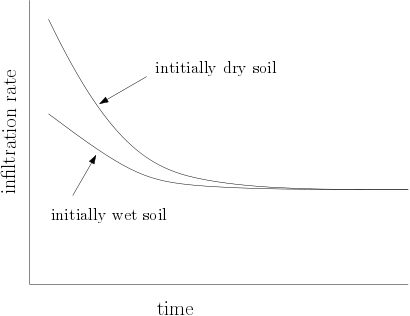
\includegraphics[width=8cm]{infiltration_schema.png}
\caption{\label{schema_inf}Schematic representation of infiltration in dry and in a wet soil.}
\end{figure}

The asymptotically established infiltration rate that is closely related to the hydraulic conductivity at field saturation. Infiltration experiments are therefore useful to estimate the saturated hydraulic conductivity K$_\mathrm{s}$. For an idealized infiltrometer with an infinite radius (purely 1D vertical water movement) and neglible water overhead, we can assume that at full saturation in the wet soil the gradient of the hydraulic (or matric) head can be assumed to be:

\begin{equation}
\frac{dh}{dz}=0
\end{equation}

Replacing this in the Darcy-Buckingham law, we obtain:
\begin{equation}
q=-K (\frac{dh}{dz}-1)=-K(0-1)=K
\end{equation}

The main issue with the interpretation of the results of the ring infiltration measurements is the lateral flow component of the water flow, which makes the analysis of the flow problem complicated.
The lateral flow causes the stationary infiltration flow to always be higher than the infiltration capacity and the hydraulic conductivity of a soil. Stagnating layers throughout the soil affected by the infiltration also cause an overestimation of the infiltration capacity.

\begin{figure}[!h]
	\centering
	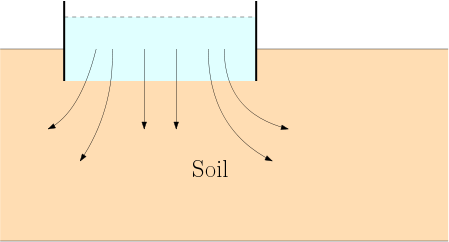
\includegraphics[width=8cm]{ring_infilt.png}
	\caption{\label{ring}Schematic of ring infiltration with lateral flow.}
\end{figure}


To avoid lateral flow double ring infiltrometer can be used. However, especially in organic soils or forest soils, they can cause unnecessary preferential flow paths. Generally, it is preferable to use rings with a large radius to have a better ratio between ring and experimental area. Using a large enough ring leads to improvement in the representativeness and can compensate for small heterogeneities.

The infiltration curve against time can be described with the 2-parametric equation according to Phillips \cite{philip1957}:

\begin{equation}\label{eq_P}
\begin{split}
I(t)&= S\cdot t^{1/2}+A\cdot t +C \\
i(t)&= S0.5 \cdot S \cdot t^{-1/2}+A.
\end{split}
\end{equation}
The constant $C$ describes the initial state of $C=0$. $S$ is the sorptivity [cm d$^{-\frac{1}{2}}$].
The infiltration rate i for t $\rightarrow$ $\infty$ is $A$. The constant $A$ [cm d$^{-1}$] is therefore with a small overhead $A=K_\mathrm{s}$. Both Parameters A and S can be determined by fitting the infiltration data to Eq. \ref{eq_P}.

To compensate for lateral flow and the overcompensation \cite{wu1997generalized} identified scaling factors, so that:

\begin{equation}\label{eq_wu}
i(t)= f K_s
\end{equation}

where $f$ is the appropriate scaling factor. $f$ can be computed using 

\begin{equation}\label{eq_wuf}
f=\frac{H+\phi_m/K_s}{y+r/2}+1
\end{equation}

where $H$ is the height of the water column above the soil, $\phi_m$ is the matric flux potential defining the influence of the water absorption through the unsaturated soil, z is the installation depth and r is the radius of the infiltration ring. Some values of f can be found in Tab.

\begin{table}[!h]
	\centering
	\caption{\label{tab_heat}Values for the scaling factor f Eq. \ref{eq_wuf} \cite{wu1997generalized}. The values are for z=5cm,H=5cm and an initial pressure head of pF=3.}
	\adjustbox{max height=\dimexpr\textheight-2cm\relax,
		max width=\textwidth}{
		
		\small\begin{tabular}{l c }
			\hline
			Soil & r=10cm\\
			\hline
			
			Fine sand & 2.6 \\
			Loam & 1.9-2.1 \\
			Clay & 3.2 \\
			\hline
		\end{tabular}
	}
\end{table}

\subsection{Ring infiltration experiment}

\begin{enumerate}
	\item Installation of ring 
	\item Measurement of diameter of ring
	\item Installation of water supply and water height regulation
	\item Beginn of experiment:
	\begin{enumerate}
		\item Read water level in the Mariotte's bottle every 30 s.
		\item The experiment end when the infiltration is stationary.
	\end{enumerate}
\end{enumerate}


\subsection{Evaluation}
We measure cumulative infiltration $I$ [cm] as the Volume entering the specific area as a function of time. 
 \begin{equation}\label{eq_infSR}
 \Delta V= \pi r^2 \delta h
 \end{equation}
 where r is the radius of the Mariotte's bottle and $\delta h$ is the water height difference in regard to the initial value.
 \begin{equation}\label{eq_infSR}
I(t) =\frac{\Delta V}{A}
 \end{equation}
The infiltration rate can be calculated as:
 \begin{equation}\label{eq_infSR}
 i = \frac{dI}{dt}\approx\frac{\Delta I}{\Delta t}
 \end{equation}

To evaluate we can plot the infiltration rate against time and fit the Phillip's equation to estimate Sorptivity $S$ and the final infiltration rate $i_f$. The saturated conductivity can be estimated using the correction factor f. 

\section{Guelph Permeameter}

The Guelph Permeameter can be used to estimate the near-surface hydraulic conductivity. The Guelph Permeameter creates a constant head and requires only approx. 2 Liter per experiment. Known problems occur with soils that show silting, where the $K_s$ will be underestimated, whereas with  layered soils $K_s$ will be overestimated. 

\begin{figure}
	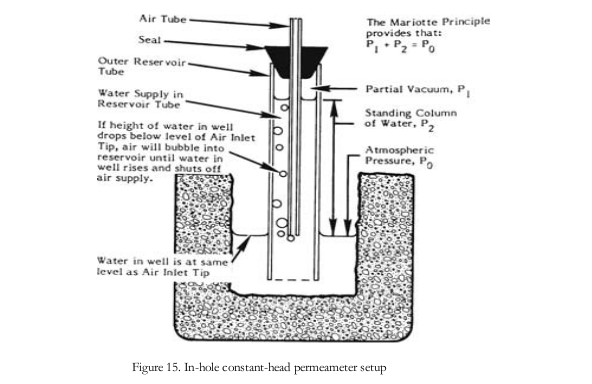
\includegraphics[width=8cm]{perm_how.png}
	\caption{Set-up of in-hole Guelph permeameter \cite{guelph_eil}.}
\end{figure}
 
 \subsection{Experiment}
 \begin{enumerate}
 	\item Create bore hole
 	\item Installation of permeameter and topping up of permeameter 
 	\item Setting of the constant head with the air entry valve
 	\item Begin experiment by opening air entry valve
 \end{enumerate}
 
 \subsection{Evaluation}
%---------------------S-------------------------------------------------------------------
%	BIBLIOGRAPHY
%----------------------------------------------------------------------------------------

%\renewcommand{\refname}{\spacedlowsmallcaps{References}} % For modifying the bibliography heading

\bibliographystyle{unsrt}

\bibliography{infilt.bib} % The file containing the bibliography

%----------------------------------------------------------------------------------------

\end{document}